\section{Avionics}\label{sec:avi} %Paul, Markus, Lukas

It is advised to read section \ref{sec:software} in 
advance to fully comprehend the following content.

\subsection{Subsystem Block Diagram (SSBD)}
The avionics subsystem is divided into multiple different modules as shown in \cref{fig:avi_ssbd}. 
Those include the three custom designed ARM based units: ECU (engine control unit), PMU (power management unit) and RCU (radio control unit), two COTS Altimax G4 altimeter as well as the mandatory Eggtimer TRS. 

\begin{figure}[H]
    \centering
    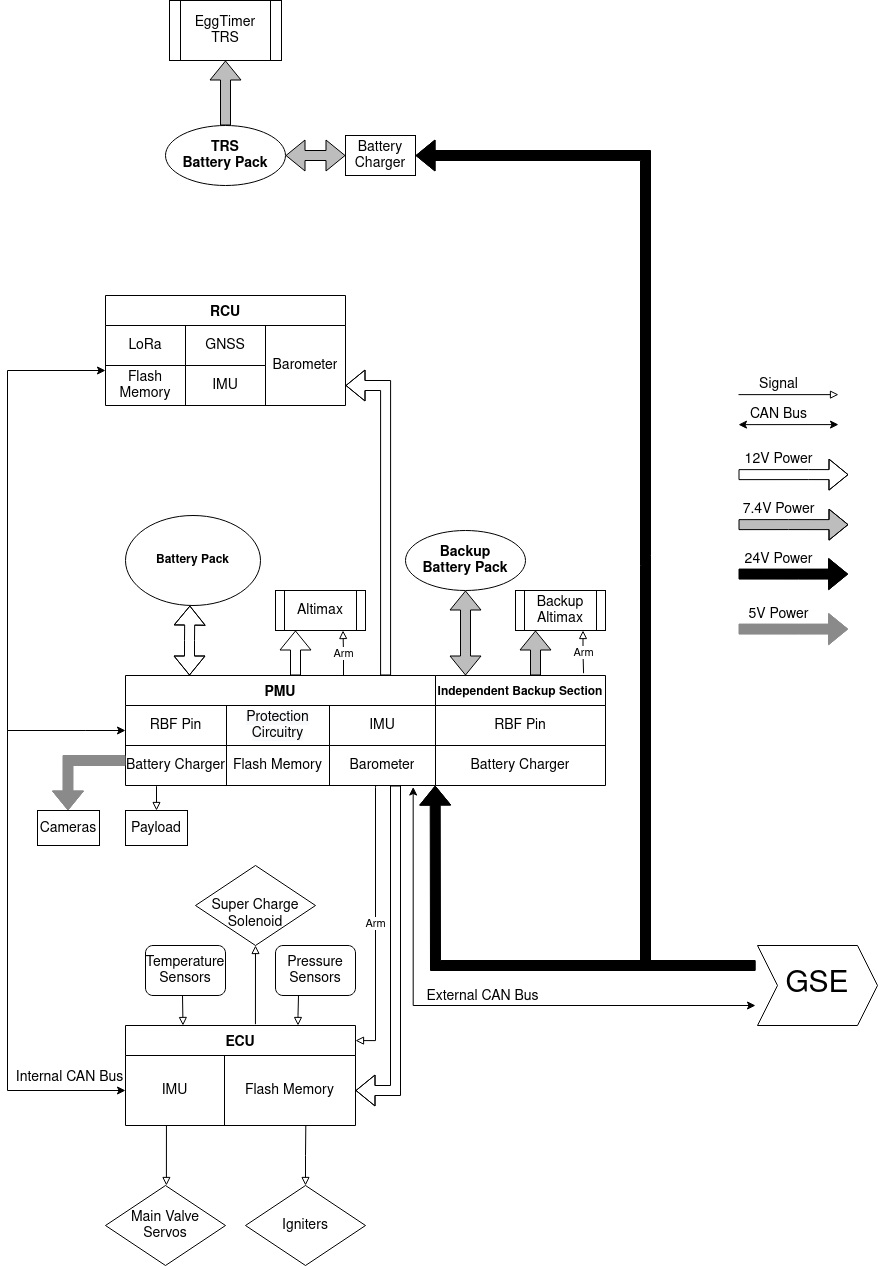
\includegraphics[scale=0.4]{Avionics/Avionics_Blockdiagram.png}
    \caption{Subsystem Block Diagram, see \cref{fig:gse_ssbd} for the block diagram for the GSE}
    \label{fig:avi_ssbd}
\end{figure}

\subsection{Physical Architecture}
The following section describes our three custom units, all equipped with an ARM processor and two CAN-FD interfaces: \textbf{ECU}, \textbf{PMU} and \textbf{RCU}.

The ECU (engine control unit) contains all the electronics necessary for the liquid propulsion system. This includes circuitry for controlling the main valve servos, the supercharge solenoid as well as the igniters. It also has inputs for the chamber and tank pressure sensors, for the tank temperature sensors and current and servo position feedback. A \SI{32}{\mega\bit} external NOR-flash-chip allows for the logging of all data packets sent to mission control in full sampling speed. This is especially useful during flight, where the data transmission speed is limited by the LoRa communication.

The PMU (power management unit) is powered by a 3S1P Li-Ion 18650 and features over-current protection, voltage and current monitoring. It also contains an IMU and a barometric pressure sensor for redundancy reasons, and logs all its data to flash memory. The PMU interfaces with all the other avionics, supplies them with power and bridges between the two CAN-FD busses. Located on a separated part of the PCB, an independent backup section powered by a backup battery pack charges and arms the backup Altimax Altimeter. Moreover, the PMUs RBF (Remove before Flight) pin circuit switches on the igniter voltage, carried to the ECU on its own power cable, separately, allowing an ECU power-up without ignition capability and, thus, ensuring that the ECU can not activate the igniters in operation modes, where the pad crew is present.

The RCU (radio communication unit) consists of communication and sensing hardware. A GNSS module, an IMU and a barometric pressure sensor collect important data for recovery and post processing. Again, all data is logged to external flash memory. A \SI{433}{\mega\hertz} LoRa module sends data to the ground station.

\subsection{Operational modes}

Safe:
Once the rocket is mounted the RBF pin is pulled halfway, which powers on all avionics onboard. At this point data is redundantly sent via \SI{433}{\mega\hertz} LoRa and the rocket can be fully controlled by our Mission Control software via a \SI{2.4}{\giga\hertz} directed radio link, the only exception being the ignition, which is still physically disconnected from power by the RBF pin. Thus,  the final pad preparations including fueling and preparing oxidizer filling are done in this mode.

Armed:
Once the on-pad preparations are done and the pad area is vacated, the RBF pin is pulled out completely, which exposes the ignition circuitry to power. The whole system is now operational. When the launch window opens oxidizer filling begins, marking the last event before launch.

Internal Control:
After oxidizer loading is completed the rocket is put into internal control, where the ECU begins its internal sequence.

Holddown:
If neither hold nor abort is commanded by the operator or the ECU, the ignition sequence is automatically started. After ignition the holddown clamps are still engaged holding the rocket firmly on the launchpad. The rocket stays in holddown mode until sufficient engine performance is detected by measuring combustion chamber pressure.

Lift-off:
If suitable chamber pressure is detected by the ECU, it commands the launch pad to release the holddown clamp. The rocket leaves the launchpad, disconnecting the electrical umbilical cord, and, thus, the power and CAN connection to the launch pad. This leaves us with only the unidirectional LoRa communication. The rocket is now fully controlled by the ECU. 

Powered Ascent:
During the powered ascent phase, data is being sent to Mission Control at all times. At the end of the planned burn time, the ECU closes the main valves to shut down the engine, also known as Main Engine Cutoff (MECO).

Unpowered Ascent:
With the ECU having finished it's internal sequence, the SRAD avionics only remain active to transmit data, shifting focus towards the COTS altimeters detecting apogee.

Recovery:
Once apogee is detected, the two-phase recovery begins with the ejection of the nose cone and drogue chute. This marks the last operation mode of the rocket. See \cref{sec:recovery} for more details on the recovery process.

\subsubsection{Pre-Launch Sequence}

The Pre-Launch Sequence is conducted on our self developed Web-Client.
It contains a dynamic and interactive Piping and Instrumentation Diagram (P\&ID/PnID) for monitoring and controlling all components, the tanking system as well as avionics inside the rocket. A checklist is carefully being processed that states each step needed for preparing and tanking the rocket for launch. Each step is announced by the Launch Commander and is re-validated and executed manually by Mission Control. At T-10 seconds internal control is activated and the rocket self-checks for any malfunctions during engine startup and launch.

\subsubsection{Abort Sequence}

In case of any malfunctions during engine startup either the internal control system can abort or Mission Control can send an abort to the rocket manually. In either case the main valves are instantly closed to prevent any thrust generation. After that a separate checklist is conducted manually to revert the system back to a safe state.

\subsubsection{CAN protocol}

To establish a steady communication with ground systems as well as the rocket, the CAN-FD protocol is used. The whole setup is split into three busses that are all connected to an Ubuntu server. Since the CAN bus is disconnected from the rocket at lift-off, a separate internal CAN bus is used to maintain communication between ECU, RCU and PMU. The PMU is able to bridge CAN messages between the internal and external CAN busses. A self developed protocol is used on top of the CAN-FD protocol to establish the controllability and flexibility needed for Mission Control.

%\subsection{Failure Analysis}

%\subsubsection{Module failure scenarios}


%\subsubsection{Testing strategies}